\documentclass{beamer}
\usetheme{metropolis}
\usepackage{graphicx}
\usepackage{subfig}
\usepackage{tcolorbox}
\title{Calculus-Based Physics-2: Electricity, Magnetism, and Thermodynamics (PHYS180-02): Unit 4}
\author{Jordan Hanson}
\institute{Whittier College Department of Physics and Astronomy}

\begin{document}
\maketitle

\section{Unit 3 Review}

\begin{frame}{Unit 3 Summary}
\textbf{Reading: Chapters 5-7}
\begin{enumerate}
\item Charge, Conductors and Insulators
\item Coulomb's Law and Electric Fields
\item E-fields of Charge Distributions
\item Gauss's Law
\end{enumerate}
\end{frame}

\section{Unit 3 Review Problems}

\begin{frame}{Unit 3 Review Problems}
Suppose a charge $q$ is located at the origin.  Use Gauss' law to find the electric field.  What is the electric field?
\begin{itemize}
\item A: $\vec{E} = \frac{kq}{r}\hat{r}$
\item B: $\vec{E} = \frac{kq}{r^2}\hat{r}$
\item C: $\vec{E} = \frac{kq}{r^3}\hat{r}$
\item D: $\vec{E} = \frac{kq^2}{r^2}\hat{r}$
\end{itemize}
\end{frame}

\begin{frame}{Unit 3 Review Problems}
Suppose a line of charge runs up the z-axis.  The charge per unit length is $\lambda$.  Use Gauss' law to find the electric field.  What is the electric field at a point $P = (x,0,0)$?
\begin{itemize}
\item A: $\vec{E} = \frac{2k\lambda}{r^2}$
\item B: $\vec{E} = \frac{2k\lambda^2}{r^2}$
\item C: $\vec{E} = \frac{2k\lambda}{r}$
\item D: $\vec{E} = 0$
\end{itemize}
\end{frame}

\section{Summary}

\begin{frame}{Unit 4 Summary}
\textbf{Reading: Chapters 7, 9, and 10}
\begin{enumerate}
\item \alert{Voltage and Capacitance}
\item Ohm's Law
\item DC circuits
\end{enumerate}
\end{frame}

\section{JITT 1.7}

\begin{frame}{JITT 1.5}
\begin{enumerate}
\item Suppose we have two charged plates, one with +Q and one with -Q, with a uniform electric field E in between them.  If the distance between the plates is d, what is the voltage difference between the plates?
\item Form an analogy between voltage and potential energy from kinematics.  In this analogy, what kinematic quantity is analogous to electric field?
\item Explain in your own works how the \alert{gradient} of a \alert{scalar field} is calculated, and how it relates to voltage and E-fields.
\end{enumerate}
\end{frame}

\begin{frame}{JITT 1.5}
\textbf{Suppose we have two charged plates, one with +Q and one with -Q, with a uniform electric field E in between them.  If the distance between the plates is d, what is the voltage difference between the plates?} \\
``you would use the equation Q=CV to find the voltage difference between the plates.'' \\
``delta V= delta U/ Q'' \\
``The voltage difference would be +Q-Q.''
\end{frame}

\begin{frame}{JITT 1.5}
\textbf{Form an analogy between voltage and potential energy from kinematics.  In this analogy, what kinematic quantity is analogous to electric field?} \\
``Voltage is similar to potential energy in that voltage is the potential change in charge and potential energy is the potential change in velocity. The electric field of a voltage would be similar to the gravity of a potential energy.'' \\
``voltage is the electric potential difference, or the possible difference between two charges. This is similar to potential energy because potential energy is the possible amount of energy of an object. Gravity would be the kinematic equivalent to electric fields.'' \\
\end{frame}

\begin{frame}{JITT 1.5}
\textbf{Explain in your own works how the \alert{gradient} of a \alert{scalar field} is calculated, and how it relates to voltage and E-fields.} \\
``you differentiate the relationship between (delta)V (this is Voltage)  and (delta)s (this is distance). deltaV/deltas = Electric field.'' \\ \vspace{0.5cm}
Let a scalar field be $U(x,y,z)$.  The \textit{gradient} of the scalar field is
\begin{equation}
\vec{\nabla} U = \frac{\partial U}{\partial x}\hat{i} + \frac{\partial U}{\partial y}\hat{j} + \frac{\partial U}{\partial z}\hat{k}
\end{equation}
\end{frame}

\section{Voltage}

\begin{frame}{Voltage}
\alert{Voltage} is analogous to potential energy in electrostatics.  The negative derivative of potential energy U is the force F:
\begin{equation}
F = -\frac{dU}{dx}
\end{equation}
For example, if the force is $F = -mg$, and the potential energy is $U = mgy$, then 
\begin{equation}
\frac{dU}{dy} = -mg
\end{equation}
\end{frame}

\begin{frame}{Voltage}
\alert{Voltage} is analogous to potential energy in electrostatics.  The derivative of voltage V is the field E:
\begin{equation}
E = -\frac{dV}{dx}
\end{equation}
For example, if the field is $E = \sigma/\epsilon_0$, and the potential energy is $V = \sigma/\epsilon_0 x + C$, then 
\begin{equation}
\frac{dV}{dx} = \sigma/\epsilon_0
\end{equation}
\end{frame}

\begin{frame}{Voltage}
\alert{Voltage} is analogous to potential energy in electrostatics. \\ \vspace{1cm}
Potential energy is just an energy.  A \textit{potential} in mechanics is the potential energy per unit mass.  \textit{Voltage}, or \textit{electrostatic potential} is \textbf{\alert{potential energy per unit charge.}} \\ 
The Volt (V) is the unit of voltage, and it has units of 1 V = 1 J/C.
\end{frame}

\begin{frame}{Voltage}
\textbf{Group board exercise}: Show that the units of electric field (normally Newtons per Coulomb) are also Volts per meter.
\end{frame}

\begin{frame}{Voltage}
\small
If the potential energy is a function of displacement, $U = U(\vec{x})$, it may be called a potential energy \textit{surface}.
\begin{figure}
\centering
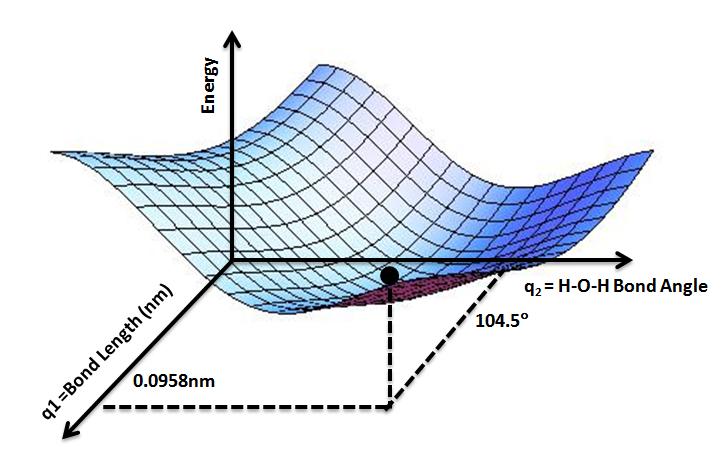
\includegraphics[width=0.5\textwidth]{figures/potential.png}
\caption{\label{fig:potential} An example of a potential energy surface.}
\end{figure}
\end{frame}

\begin{frame}{Voltage}
\small
Considering \textit{Newton's Second Law}, however, if $F = m a$ then $m a = -\frac{\Delta U}{\Delta x}$, and
\begin{equation}
a = -\frac{1}{m}\frac{\Delta U}{\Delta x} \label{eq:field}
\end{equation}
\begin{figure}
\centering
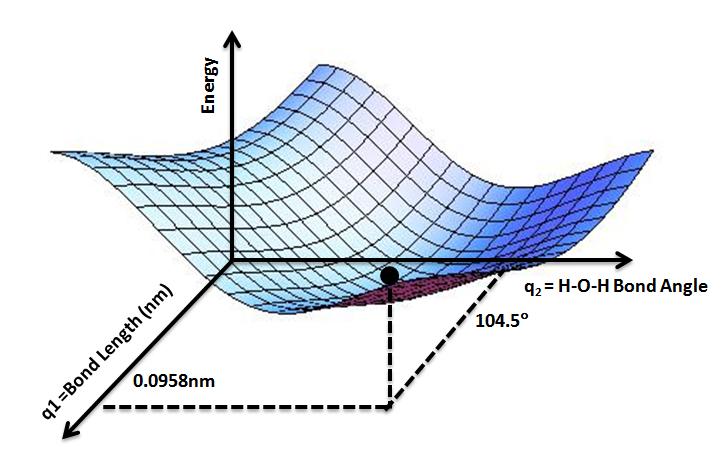
\includegraphics[width=0.4\textwidth]{figures/potential.png}
\caption{\label{fig:potential2} If we divide by the mass we have acceleration.}
\end{figure}
The derivative, or \textit{gradient}, of $a$ in Eq. \ref{eq:field} is analogous to the electric field.  But the electric field is a \textit{vector field}...
\end{frame}

\begin{frame}{Voltage}
The gradient is like a derivative, but gives you the proper direction wherever you are.
\begin{equation}
\boxed{
\vec{\nabla} V = \vec{E} = -\frac{\partial V}{\partial x}\hat{i}-\frac{\partial V}{\partial y}\hat{j}-\frac{\partial V}{\partial z}\hat{k}}
\end{equation}
\end{frame}

\begin{frame}{Unit 3 Review Problems}
Suppose the voltage due to some charge distribution is $V(x,y,z) = ax+b$.  What is the field?
\begin{itemize}
\item A: $\vec{E} = a\hat{j}$
\item B: $\vec{E} = a\hat{k}$
\item C: $\vec{E} = b\hat{i}$
\item D: $\vec{E} = a\hat{i}$
\end{itemize}
\end{frame}

\begin{frame}{Unit 3 Review Problems}
Suppose the voltage due to some charge distribution is $V(x,y,z) = ax+by$.  What is the field?
\begin{itemize}
\item A: $\vec{E} = -a\hat{j}-b\hat{j}$
\item B: $\vec{E} = a\hat{k}+b\hat{k}$
\item C: $\vec{E} = -b\hat{i}-a\hat{j}$
\item D: $\vec{E} = -a\hat{i}-b\hat{j}$
\end{itemize}
\end{frame}

\begin{frame}{Voltage}
Suppose a charge distribution is made of two infinite plates of charge with charge per unit area $\pm\sigma$.  We know that the field is $\sigma/\epsilon_0 \hat{k}$ between them.  \textbf{Group board exercise}: Draw the charge distribution, define a coordinate system, and write the function for the voltage.
\end{frame}

\begin{frame}{Voltage}
\textbf{Voltage} is like a potential energy surface $\rightarrow$ \textit{potential energy per unit charge.} \\ \vspace{0.5cm}
\url{https://phet.colorado.edu/en/simulation/charges-and-fields} \\
\alert{Using the PhET simulation about charges and fields}:
\begin{enumerate}
\item Explore the voltage associated with fields generated by charges using the voltage button.
\item Add a single point charge, and use the ruler and voltmeter (potentiometer) to measure voltage versus distance, and plot it.
\item What function describes the relationship between voltage and distance?
\end{enumerate}
\end{frame}

\begin{frame}{Voltage}
\url{https://phet.colorado.edu/en/simulation/charges-and-fields} \\
\alert{Using the PhET simulation about charges and fields}:
\begin{enumerate}
\item Note that the units of $\epsilon_0$ are N m$^2$ C$^{-2}$, and the value is $8.854\times 10^{-12}$
\item We know from prior equations that the units of voltage are J C$^{-1}$
\item Using your measurements, show that the voltage due to a point charge is
\begin{equation}
\boxed{
V = \pm \frac{1}{4\pi \epsilon_0} \frac{q}{r}}
\end{equation}
(Where the sign depends on the charge, just like E-fields)
\end{enumerate}
\end{frame}

\begin{frame}{Voltage}
Voltage due to a point charge:
\begin{equation}
\boxed{
V = \pm \frac{1}{4\pi \epsilon_0} \frac{q}{r}} \label{eq:volt2}
\end{equation}
\end{frame}

\begin{frame}{Voltage}
Voltage is an example of a \textbf{scalar field}, whereas the electric field is an example of a \textbf{vector field.}  Create two lines of charge, one positive and one negative in the PHeT simulator, and pretend they represent planes of charge coming out of the screen.  The field should constant and uniform like
\begin{equation}
\vec{E} = \frac{\sigma}{\epsilon_0} \hat{k}
\end{equation}
\begin{enumerate}
\item Plot the voltage versus distance between the plates.
\item Calculate the slope in V/m, and the y-intercept in V.
\item Does the electric field depend on the y-intercept?  Does the charge distribution?
\end{enumerate}
\end{frame}

\begin{frame}{Voltage}
\begin{figure}
\centering
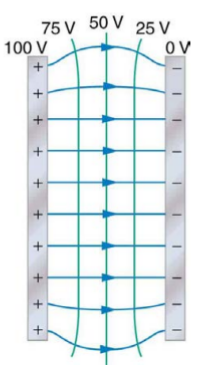
\includegraphics[width=0.25\textwidth]{figures/plates.png}
\caption{\label{fig:plates} Parallel plates of charge, electric field, and potential.  Notice the linear decrease in voltage.}
\end{figure}
\textbf{How we define the y-intercept in voltage is analogous to the zero-point freedom of potential energy.}
\end{frame}

\begin{frame}{Voltage}
\textit{Two parallel plates, opposite charge}:
\begin{equation}
V = -\frac{\sigma}{\epsilon_0}z + C
\end{equation}
With the boundary condition that $V = V_0$ when $z = 0$, we have
\begin{equation}
V(z) - V_0 = -\frac{\sigma}{\epsilon_0}z
\end{equation}
Let $\Delta V(z) = V(z) - V_0$, and $\Delta z = z$:
\begin{equation}
-\frac{\Delta V}{\Delta z} = \frac{\sigma}{\epsilon_0} =  E
\end{equation}
\end{frame}

\begin{frame}{Voltage}
\textbf{Continuing with PHeT:} Make a ring of charge that has a radius of 100 cm, with the center at the origin.
\begin{enumerate}
\item Show that the voltage field is radially symmetric.
\begin{itemize}
\item Place \textit{equipotential lines} around the charge distribution and see that they are circular.
\end{itemize}
\item Show that at distances much larger than the radius, the voltage field looks like that of a point charge.
\begin{itemize}
\item Record the voltage versus distance from the origin.
\item Plot the data.
\item Compare to the plot corresponding to a point charge.
\end{itemize}
\end{enumerate} 
\end{frame}

\begin{frame}{Voltage}
Now that we know that only voltage \textit{differences} matter:
\begin{equation}
\Delta V = - \int \vec{E} \cdot \vec{dl}
\end{equation}
What else is analogous to potential energy?
\end{frame}

\begin{frame}{Voltage}
Suppose the voltage due to some charge distribution is $V$.  What is the voltage difference if when we try to integrate like:
\begin{equation}
\Delta V = - \oint \vec{E} \cdot \vec{dl}
\end{equation}
\begin{itemize}
\item A: $\Delta V = E \cdot L$
\item B: $\Delta V = 0$
\item C: $\Delta V = E dl$
\item D: $\Delta V = L$
\end{itemize}
\end{frame}

\begin{frame}{Voltage}
The previous question reminds us that electric fields are \textbf{conservative.}
\end{frame}

\begin{frame}{Voltage}
The voltage of a point charge $+q$ is $V = \frac{kq}{r}$.  What is the electric field?
\begin{itemize}
\item A: $\frac{kq}{r}$
\item B: $\frac{kq}{r^2}$
\item C: $\frac{kq^2}{r}$
\item D: $\frac{kq^2}{r^2}$
\end{itemize}
\end{frame}

\begin{frame}{Voltage}
What happened to the minus sign in the last problem?
\begin{itemize}
\item A: It disappeared...because.
\item B: Only voltage differences matter.
\item C: The zero-point of the voltage is at infinity.
\item D: It's cancelled by the definition: negative derivative of voltage is E-field.
\end{itemize}
\end{frame}

\begin{frame}{Voltage}
The electric field of a long line of charge with charge density $\lambda$ is $\vec{E} = \frac{2k\lambda}{r}\hat{r}$.  What is the voltage?
\begin{itemize}
\item A: $\frac{2k\lambda}{r^2}$
\item B: $\frac{4k\lambda}{r^2}$
\item C: $2k\lambda^2\ln(r) + V_0$
\item D: $-2k\lambda\ln(r) + V_0$
\end{itemize}
\end{frame}

\begin{frame}{Voltage}
\textbf{Line integral example}: view on board.
\begin{equation}
\Delta V = -\int \vec{E} \cdot \vec{dl}
\end{equation}
Once the path is specified, we can perform this integral: \url{https://en.wikipedia.org/wiki/Line_integral}
\end{frame}

\section{Units of Energy}

\begin{frame}{Units of Energy}
The electron-volt: eV.  This is the energy gained by an electron accelerated through a voltage of 1 V.
\begin{itemize}
\item How many Joules per electron volt?
\item What is the mass of a proton in eV? (E = mc$^2$, where $c$ is the speed of light.)
\end{itemize}
\end{frame}

\begin{frame}{Units of Energy}
A proton is released into a 40 kV electric potential.  What is the final kinetic energy of the proton?
\begin{itemize}
\item A: -20 kV
\item B: 40 kV
\item C: -40 keV
\item D: 40 keV
\end{itemize}
\end{frame}

\section{Capacitance}

\begin{frame}{Capacitance}
\textbf{Capacitance} is the ability of an object to store charge.  Let the voltage difference across an object be $V$, storing $-Q$ on one side and $+Q$ on another.  The \textit{capacitance} $C$ is given by
\begin{equation}
Q = C V
\end{equation}
Let the object be two parallel plates, and the charges be $\pm Q$.
\end{frame}

\begin{frame}{Capacitance}
\begin{figure}
\centering
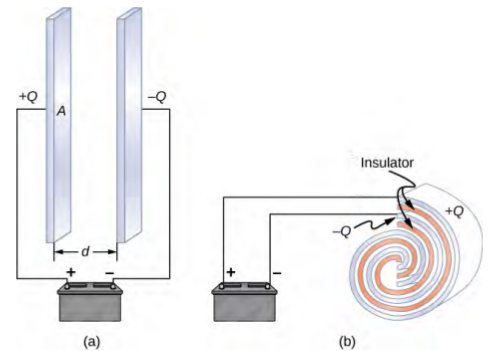
\includegraphics[width=0.8\textwidth]{figures/cap.png}
\caption{\label{fig:cap} General scheme of a capacitor.}
\end{figure}
\end{frame}

\begin{frame}{Capacitance}
The electric field and voltage between two charged plates separated by a distance $d$ is $V = Ed$.  The field is $E = \sigma/\epsilon_0$, and $Q = \sigma/A$, where $A$ is the plate area and $\sigma$ is the surface charged density.  Note that
\begin{align}
C = Q/V &= (Q)/(E d) \\
= (Q \epsilon_0)/(\sigma d) &= (Q A \epsilon_0)/(Q d) \\
= \frac{A \epsilon_0}{d} &
\end{align}
So the capacitance depends on the permittivity of free space, the area, and the distance.  In other words, just the geometry of the system.  The units of capcitance are \textbf{\alert{Farads}} (F).  This is a large unit.  Typical capacitors have nF or pF.
\end{frame}

\begin{frame}{Capacitance}
\textbf{Group board exercise}: The permittivity of free space is $8.85 \times 10^{-12}$ N$^{-1}$ C$^2$ m$^{-2}$.  A capacitor has an area of 1 mm$^2$, and $d = 0.001$ mm.  What is the capacitance? \\ 
\textbf{Group board exercise}: The permittivity of free space is $8.85 \times 10^{-12}$ N$^{-1}$ C$^2$ m$^{-2}$.  A capacitor has an area of 10 mm$^2$, and $d = 0.001$ mm.  What is the capacitance? \\
\textbf{Group board exercise}: The permittivity of free space is $8.85 \times 10^{-12}$ N$^{-1}$ C$^2$ m$^{-2}$.  A capacitor has an area of 1 mm$^2$, and $d = 0.01$ mm.  What is the capacitance?
\end{frame}

\section{Ohm's Law, Kirchhoff's Rules and Simple Circuits}

\begin{frame}{Ohm's Law, Kirchhoff's Rules and Simple Circuits}
\textbf{Read chapters 9 and 10 for Monday.}
Voltage and capacitance can be combined with another concept, \alert{resistance}, to build an understanding of \alert{circuits}.  Ohm's law is the relationship between \textit{current} and \textit{voltage}:
\begin{equation}
V = I R = \frac{dQ}{dt}R
\end{equation}
Current is the \textit{flow of charge.}  The unit of resistance is called the Ohm, and the unit of current is called the amp, for Amp\`{e}re.
\end{frame}

\begin{frame}{Ohm's Law, Kirchhoff's Rules and Simple Circuits}
A 9 V battery powers a smoke detector, and the current is 0.009 amps.  What is the resistance of the circuit powering the smoke detector?
\begin{itemize}
\item A: 1000 Ohms
\item B: 100 Ohms
\item C: 10 Ohms
\item D: 1 Ohm
\end{itemize}
\end{frame}

\begin{frame}{Ohm's Law, Kirchhoff's Rules and Simple Circuits}
A 3.3 V battery powers a christmas light, and the current is 0.33 amps.  What is the resistance of the circuit powering the smoke detector?
\begin{itemize}
\item A: 1000 Ohms
\item B: 100 Ohms
\item C: 10 Ohms
\item D: 1 Ohm
\end{itemize}
\end{frame}

\begin{frame}{Ohm's Law, Kirchhoff's Rules and Simple Circuits}
Resistors, capacitors, voltages, and current can be combined conceptually to form \alert{\textbf{DC Circuits}} (direct-current).  The following rules govern the interaction of resistors with each other, and capacitors with each other:
\begin{itemize}
\item For resistors \textit{in series}: $R = R_1 + R_2 + R_3 + ...$
\item For resistors \textit{in parallel}: $R^{-1} = R_1^{-1} + R_2^{-1} + R_3^{-1} + ...$
\item For capacitors \textit{in parallel}: $C = C_1 + C_2 + C_3 + ...$
\item For capacitors \textit{in series}: $C^{-1} = C_1^{-1} + C_2^{-1} + C_3^{-1} + ...$
\end{itemize}
\textbf{Observe on board:} difference between in series, and in parallel? (Hint, different voltage for in series, same voltage for in parallel).
\end{frame}

\begin{frame}{Ohm's Law, Kirchhoff's Rules and Simple Circuits}
Kirchhoff's rules:
\begin{enumerate}
\item Summing the voltage in a loop must equal zero ($\vec{E}$-fields are conservative).
\item Current entering an leaving a node is conserved.
\end{enumerate}
\textbf{Observe on board.}
\end{frame}

\begin{frame}{Ohm's Law, Kirchhoff's Rules and Simple Circuits}
Two resistors have 1 k$\Omega$ each (1000 Ohms).  What is the effective resistance if they are added \textit{in parallel}?
\begin{itemize}
\item A: 1000 Ohms
\item B: 500 Ohms
\item C: 2000 Ohms
\item D: 200 Ohms
\end{itemize}
\end{frame}

\begin{frame}{Ohm's Law, Kirchhoff's Rules and Simple Circuits}
Two capacitors have 1 nF each.  What is the effective capacitance if they are added \textit{in series}?
\begin{itemize}
\item A: 0.5 nF
\item B: 5 nF
\item C: 1 nF
\item D: 2 nF
\end{itemize}
\end{frame}

\begin{frame}{Ohm's Law, Kirchhoff's Rules and Simple Circuits}
Two capacitors have 1 nF each.  What is the effective capacitance if they are added \textit{in parallel}?
\begin{itemize}
\item A: 0.5 nF
\item B: 5 nF
\item C: 1 nF
\item D: 2 nF
\end{itemize}
\end{frame}

\section{Graphical Analysis of Simple Circuits}

\begin{frame}{Graphical Analysis}
\begin{columns}[T]
\begin{column}{0.5\textwidth}
\begin{figure}
\centering
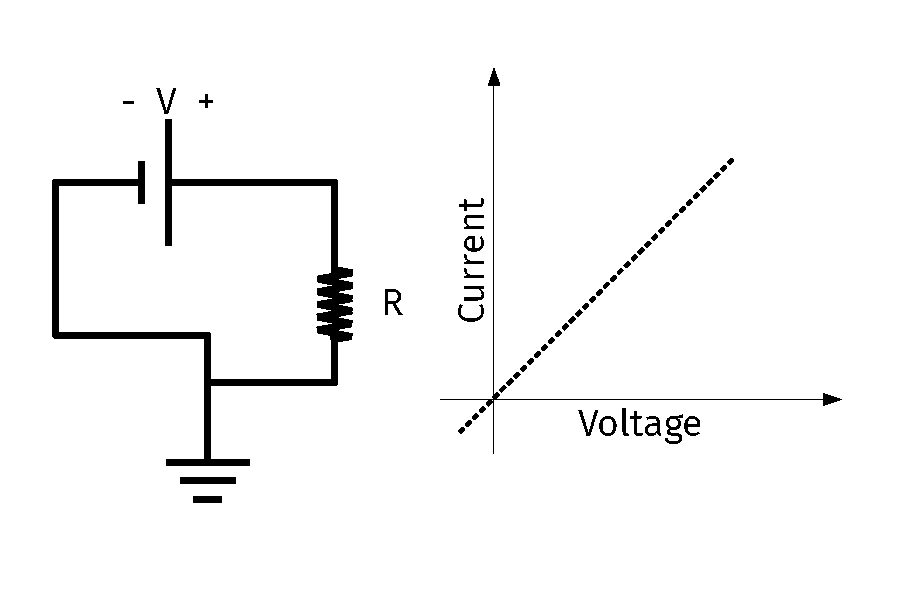
\includegraphics[width=\textwidth,trim=0.5cm 0cm 1cm 0cm,clip=true]{figures/iVCurve.pdf}
\caption{\label{fig:iVCurve1} Circuits components are represented graphically by iV curves.}
\end{figure}
\end{column}
\begin{column}{0.5\textwidth}
\small
If the resistance $R$ is increased, what will happen?
\begin{itemize}
\item A: The slope on the graph will increase
\item B: The slope on the graph will decrease
\item C: The slope will stay the same
\item D: Cannot determine what will happen
\end{itemize}
\end{column}
\end{columns}
\end{frame}

\begin{frame}{Graphical Analysis}
\begin{columns}[T]
\begin{column}{0.5\textwidth}
\begin{figure}
\centering
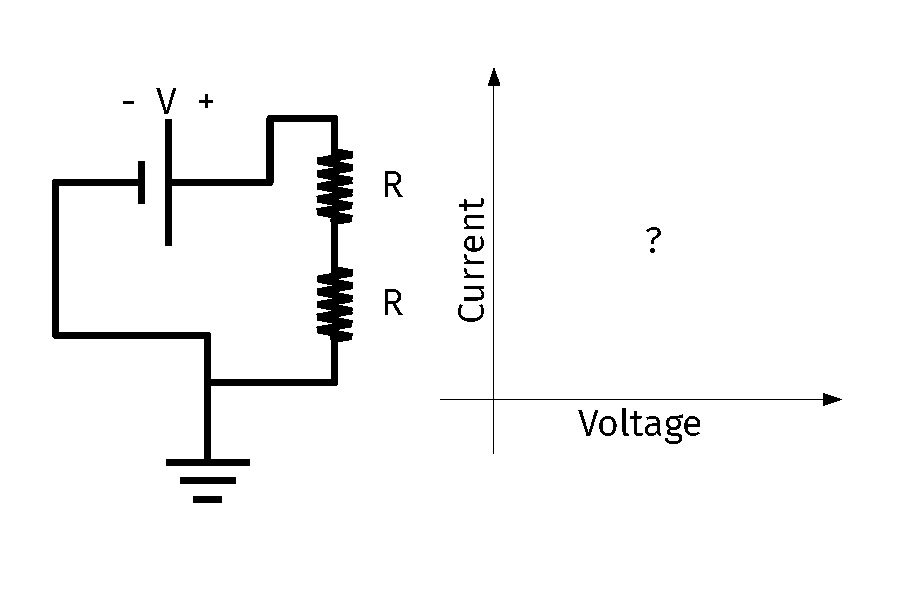
\includegraphics[width=\textwidth,trim=0.5cm 0cm 1cm 0cm,clip=true]{figures/iVCurve2.pdf}
\caption{\label{fig:iVCurve2} Circuits components are represented graphically by iV curves.}
\end{figure}
\end{column}
\begin{column}{0.5\textwidth}
\small
Should the slope now be greater than, less than, or equal to the that of Fig. \ref{fig:iVCurve1}?
\begin{itemize}
\item A: Greater than Fig. \ref{fig:iVCurve1}
\item B: Less than Fig. \ref{fig:iVCurve1}
\item C: Equal to Fig. \ref{fig:iVCurve1}
\item D: Cannot determine.
\end{itemize}
\end{column}
\end{columns}
\end{frame}

\begin{frame}{Graphical Analysis}
\begin{columns}[T]
\begin{column}{0.5\textwidth}
\begin{figure}
\centering
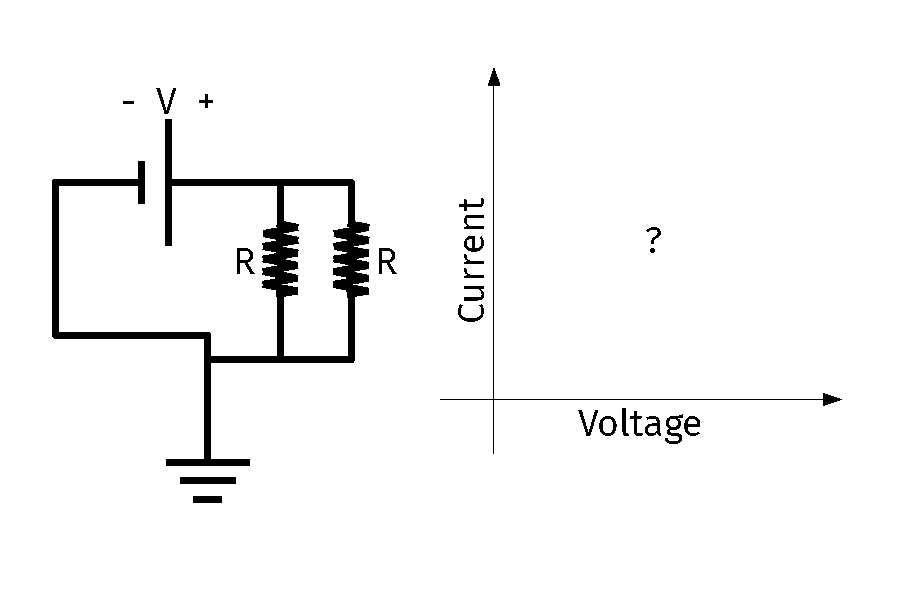
\includegraphics[width=\textwidth,trim=0.5cm 0cm 1cm 0cm,clip=true]{figures/iVCurve3.pdf}
\caption{\label{fig:iVCurve3} Circuits components are represented graphically by iV curves.}
\end{figure}
\end{column}
\begin{column}{0.5\textwidth}
\small
Should the slope now be greater than, less than, or equal to the that of Fig. \ref{fig:iVCurve1}?
\begin{itemize}
\item A: Greater than Fig. \ref{fig:iVCurve1}
\item B: Less than Fig. \ref{fig:iVCurve1}
\item C: Equal to Fig. \ref{fig:iVCurve1}
\item D: Cannot determine.
\end{itemize}
\end{column}
\end{columns}
\end{frame}

\begin{frame}{Graphical Analysis}
\begin{columns}[T]
\begin{column}{0.5\textwidth}
\begin{figure}
\centering
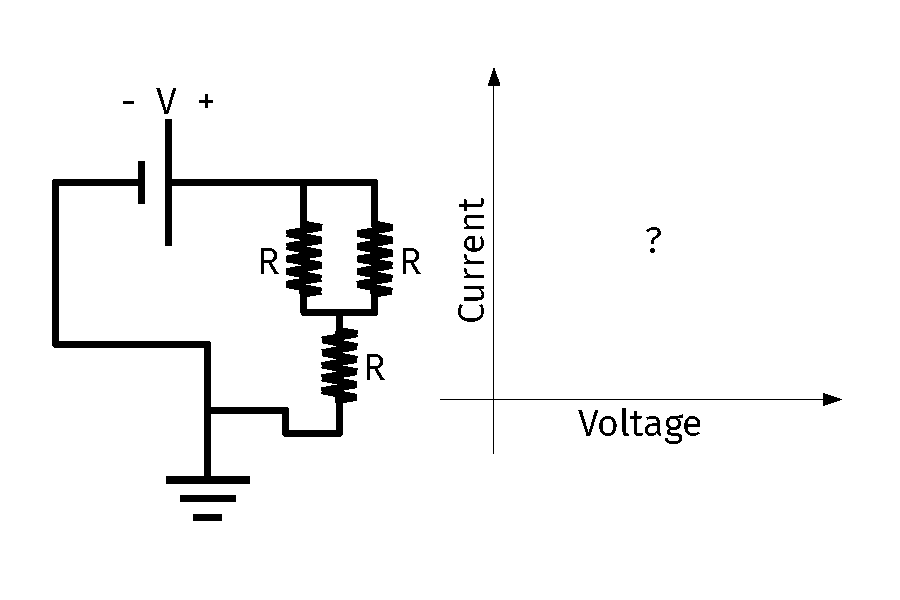
\includegraphics[width=\textwidth,trim=0.5cm 0cm 1cm 0cm,clip=true]{figures/iVCurve4.pdf}
\caption{\label{fig:iVCurve4} Circuits components are represented graphically by iV curves.}
\end{figure}
\end{column}
\begin{column}{0.5\textwidth}
\small
Should the slope now be greater than, less than, or equal to the that of Fig. \ref{fig:iVCurve1}?
\begin{itemize}
\item A: Greater than Fig. \ref{fig:iVCurve1}
\item B: Less than Fig. \ref{fig:iVCurve1}
\item C: Equal to Fig. \ref{fig:iVCurve1}
\item D: Cannot determine.
\end{itemize}
\end{column}
\end{columns}
\end{frame}

\begin{frame}{DC circuit Analysis}
\textbf{Group board exercise:} Solve for the current.
\begin{figure}
\centering
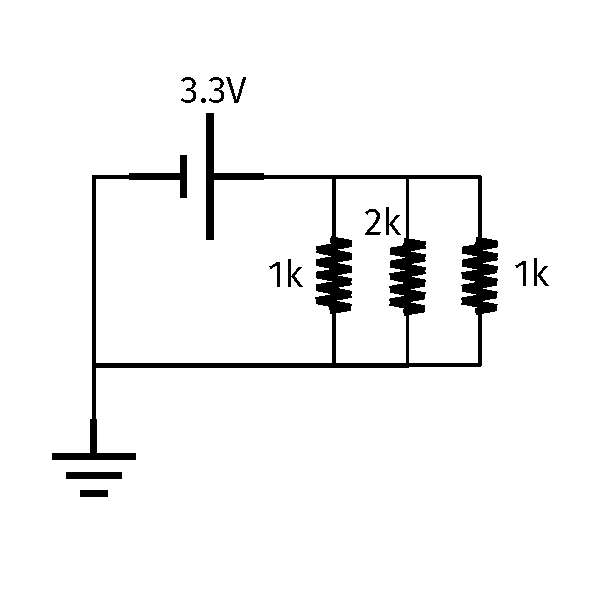
\includegraphics[width=0.5\textwidth]{figures/iVCurve5.pdf}
\caption{\label{fig:iVCurve5} Three resistors in parallel.}
\end{figure}
\end{frame}

\begin{frame}{DC circuit Analysis}
\textbf{Group board exercise:} Solve for the current.
\begin{figure}
\centering
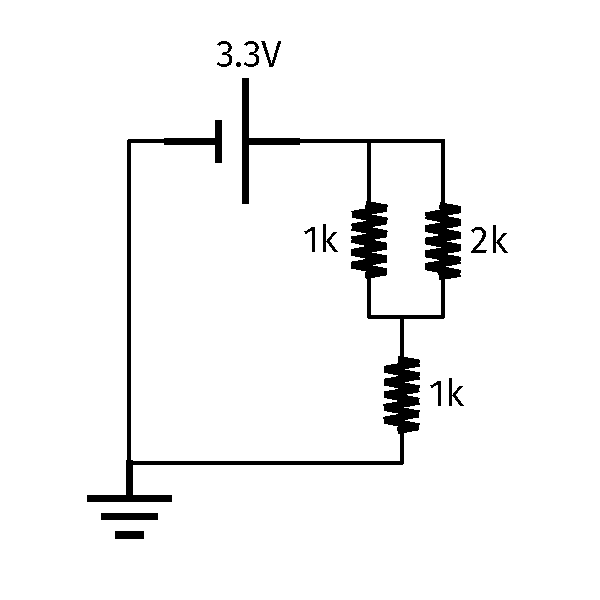
\includegraphics[width=0.5\textwidth]{figures/iVCurve6.pdf}
\caption{\label{fig:iVCurve6} Two resistors in parallel, and in series with a third.}
\end{figure}
\end{frame}

\begin{frame}{DC circuit Analysis}
\textbf{Group board exercise:} Solve for the current.
\begin{figure}
\centering
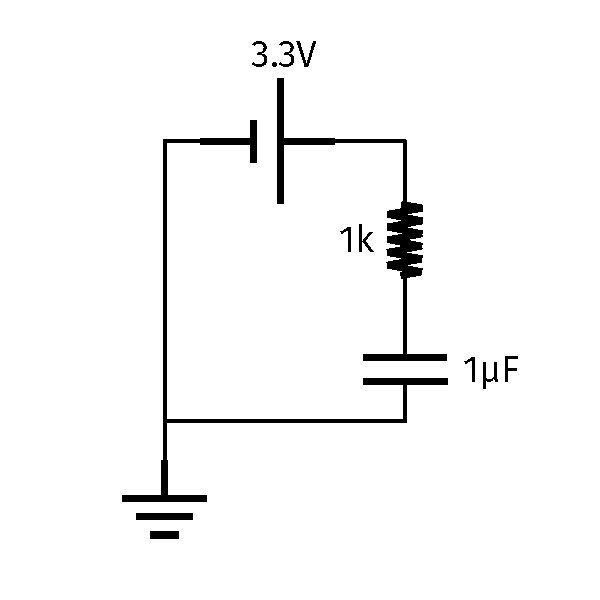
\includegraphics[width=0.5\textwidth]{figures/iVCurve7.pdf}
\caption{\label{fig:iVCurve7} A resistor in series with a capacitor...}
\end{figure}
\end{frame}

\begin{frame}{DC circuit Analysis}
Using Kirchhoff's loop rule:
\begin{align}
V - iR - QC^{-1} &= 0 \\
Q_0 &= CV \\
\tau &= RC \\
\tau \dot{Q} + Q &= Q_0
\end{align}
\textbf{Group board exercise:} Show that the solution for the charge on the capacitor is
\begin{equation}
Q(t) = Q_0 \left(1 - \exp(-t/\tau)\right)
\end{equation}
Take the derivative of both sides to find the current versus time.  Graph the current.
\end{frame}

\section{Conclusion}

\begin{frame}{Unit 4 Summary}
\textbf{Reading: Chapters 7, 9, and 10}
\begin{enumerate}
\item \alert{Voltage and Capacitance}
\item Ohm's Law
\item DC circuits
\end{enumerate}
\end{frame}

\section{Answers}

\begin{frame}{Answers}
\tiny
\begin{columns}[T]
\begin{column}{0.5\textwidth}
\begin{itemize}
\item $\vec{E} = \frac{kq}{r^2}\hat{r}$
\item $\vec{E} = \frac{2k\lambda}{r}$
\item $\vec{E} = -a\hat{i}$
\item $\vec{E} = -a\hat{i}-b\hat{j}$
\item $\Delta V = 0$
\item $\frac{kq}{r^2}$
\item D
\item $-2k\lambda\ln(r) + V_0$
\item 40 keV
\item 1000 Ohms
\item 10 Ohms
\item 500 Ohms
\item 0.5 nF
\item 2 nF
\end{itemize}
\end{column}
\begin{column}{0.5\textwidth}
\begin{itemize}
\item The slope on the graph will decrease
\item Less than Fig. \ref{fig:iVCurve1}
\item Greater than Fig. \ref{fig:iVCurve1}
\item Less than Fig. \ref{fig:iVCurve1}
\end{itemize}
\end{column}
\end{columns}
\end{frame}

\end{document}
